\section{Results} 

\subsection{Evaluation of the Knowledge Transfer Methods}
We first reproduce the zero-shot and few-shot experiments for the teacher and student architectures WRN-40-2 and WRN-16-1 on SVHN and CIFAR-10. The results are presented in Figure \ref{fig:performance}, which shows test accuracy of the baseline model KD-AT trained with $M$ samples or all data, as well as the zero-shot model and a student trained from scratch with $M$ samples. The test accuracy are the means over three trials. In addition, the results include the performance of Variational Information Distillation (VID) of \cite{Ahn2019VariationalID}. We can see in Figure \ref{fig:performance} that the results of the paper are reproduced, where the zero-shot model outperforms KD-AT and VID trained with $M=100$ samples, and almost reaches the accuracy of KD-AT with $M=5000$ on SVHN.

\begin{figure}[H]
\centering
\minipage{0.5\textwidth}%
  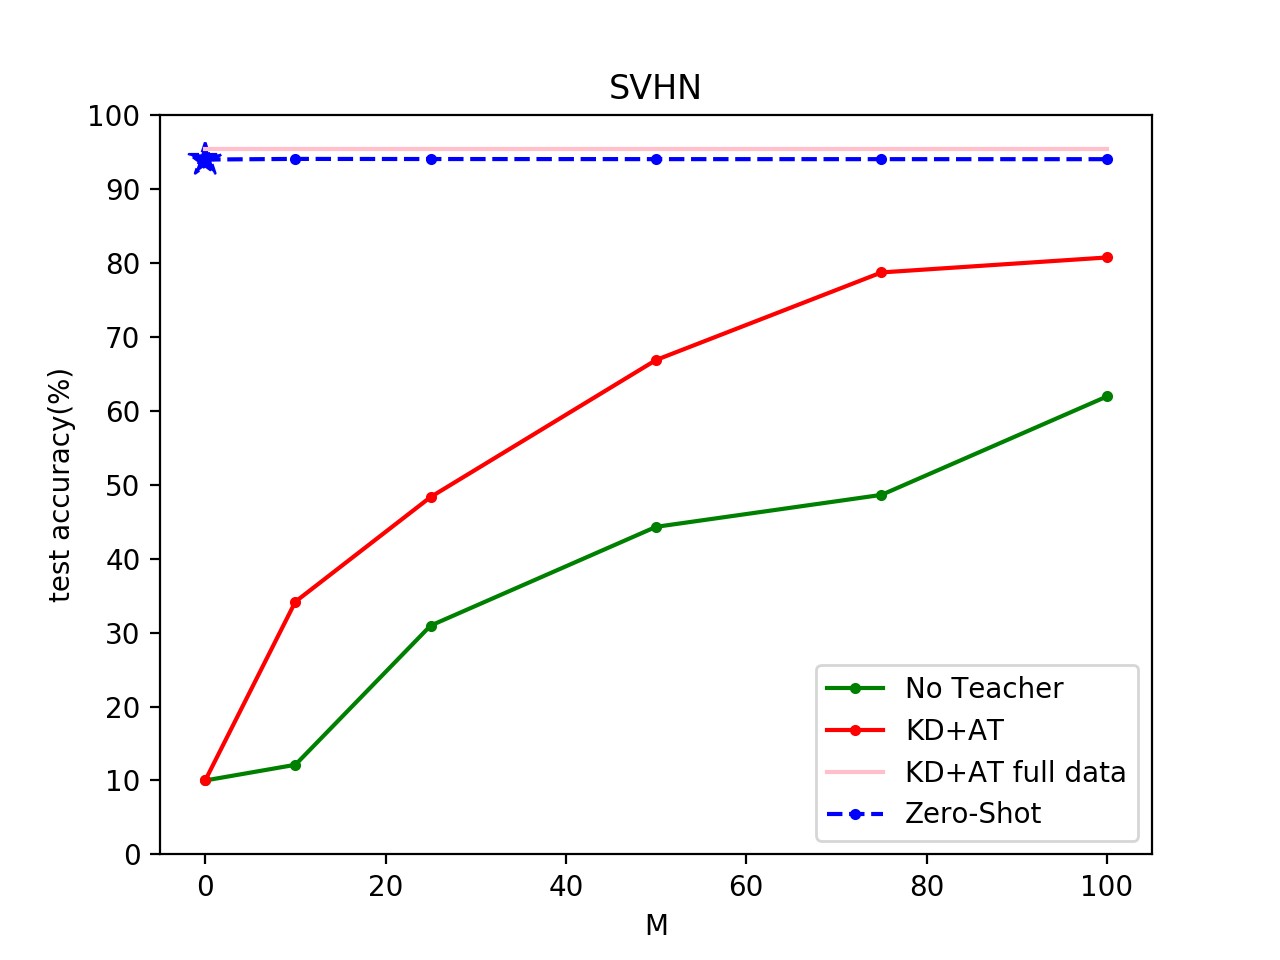
\includegraphics[width=\linewidth]{images/svhn_performance.png}
  \caption*{(a)}
  
\endminipage
\minipage{0.5\textwidth}
  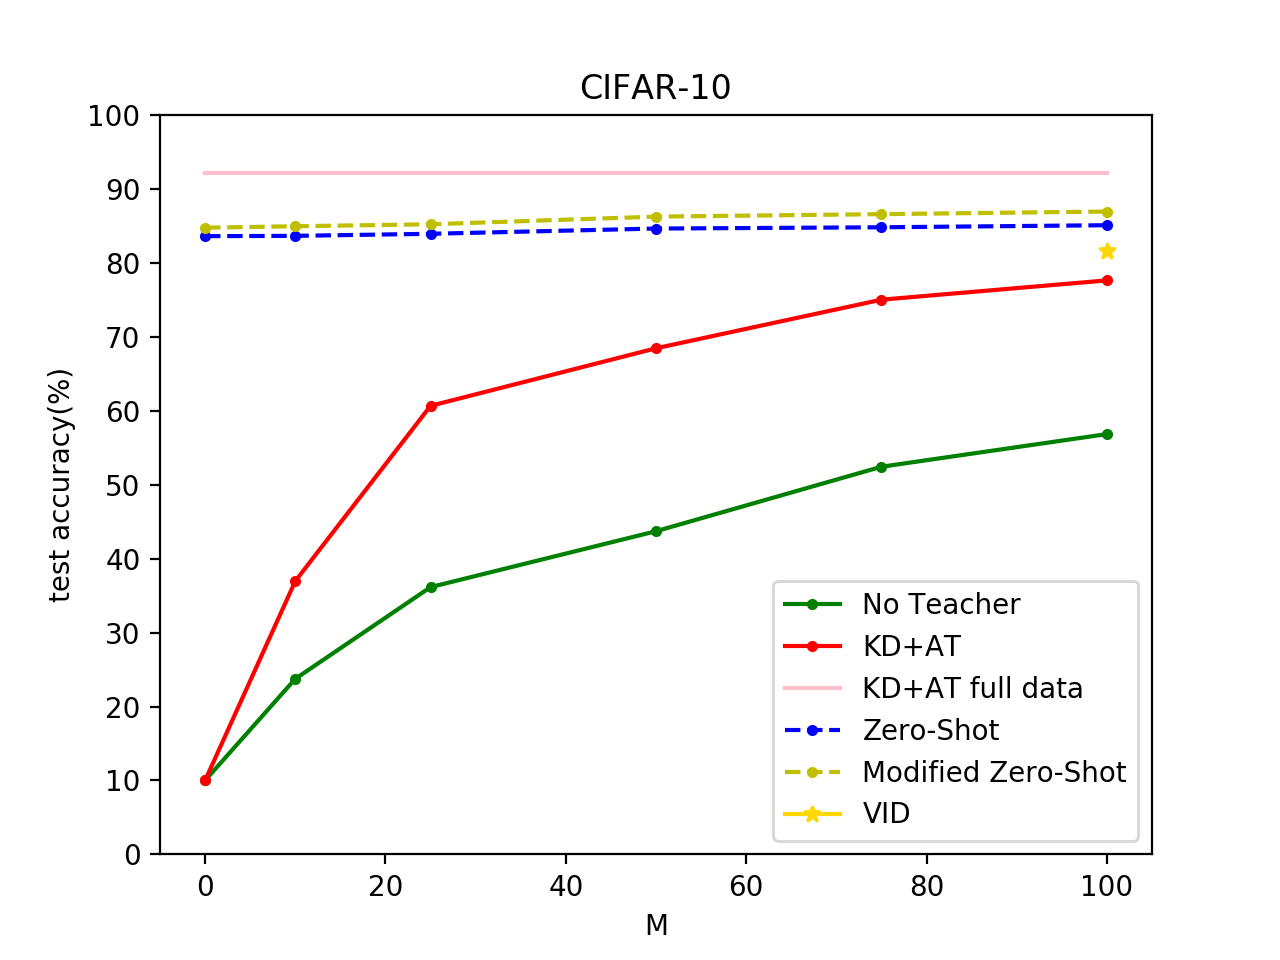
\includegraphics[width=\linewidth]{images/modified-cifar-performance.png}
  \caption*{(b)}
\endminipage\hfill

\caption{ Performance for different algorithms using SVHN (a) and CIFAR-10 (b) datasets. Variational information distillation (VID)\cite{Ahn2019VariationalID} has a single value for the CIFAR-10 dataset using M=100 samples per class.}
\label{fig:performance}
\end{figure}

Table \ref{olamesa} shows reproduced results of the experiment investigating architecture dependence on CIFAR-10. The mean test accuracy over three trials is close to the results of the paper, with small discrepancies. Similar to the official results, we also notice that the zero-shot distilling setting from WRN-40-2 to WRN-16-2 performs better than distilling from the same teacher to WRN-40-1, suggesting that deeper student networks with similar number of parameters not necessarily perform better. The opposite can be seen for KD-AT, with the deeper student network performing best (but with larger standard deviations than the paper). Moreover, we include results of our modified zero-shot algorithm, which show improved performance for all network architectures. Training our modified algorithm requires multiple generated batches per iteration, and results in higher complexity in terms of speed. However, it converges to a similar or higher accuracy in fewer iterations of the training process, making it run in a similar time or sometimes faster than the original zero-shot algorithm. Due to the complexity of the task, we did not have enough resources to further evaluate the performance of the algorithm. 

\begin{table}[!ht]
 \begin{adjustwidth}{-1.5cm}{}

    \centering
    \begin{tabular}{lc|ccccc}
    \toprule
    \toprule
         Teacher & Student & Teacher & Student & KD+AT & Zero-Shot & Modified   \\
         (\# params) & (\# params) & scratch & scratch & M = 200 &  & Zero-Shot \\
         \midrule
         WRN-16-2  & WRN-16-1  & $94.21 \pm \scriptstyle{0.03}$ & $91.38\pm \scriptstyle{0.33}$ & $85.55\pm \scriptstyle{0.25}$ & $81.25\pm \scriptstyle{0.86} $ & $82.82\pm \scriptstyle{1.09} $ \\
         WRN-40-1  & WRN-16-1 (175K) & $93.83\pm \scriptstyle{0.22}$ & $91.38\pm \scriptstyle{0.33}$ & $83.64\pm \scriptstyle{0.22}$ & $79.90\pm \scriptstyle{1.82}$ & $82.61\pm \scriptstyle{2}$\\
         WRN-40-2 (2.243M) & WRN-16-1 (175K) & $95.16\pm \scriptstyle{0.04}$ & $91.38\pm \scriptstyle{0.33}$ & $82.85\pm \scriptstyle{0.95}$  & $83.63\pm \scriptstyle{0.15}$ & $84.78\pm \scriptstyle{0.5}$\\
         WRN-40-1 (563K) & WRN-16-2 (691K) & $93.83\pm \scriptstyle{0.22}$ & $94.21\pm \scriptstyle{0.03}$ & $87.25\pm \scriptstyle{0.18}$ & $87.71\pm \scriptstyle{0.71}$ & $89.27\pm \scriptstyle{0.6}$\\ 
         WRN-40-2 (2.243M) & WRN-16-2 (691K) & $95.16\pm \scriptstyle{0.04}$ & $94.21\pm \scriptstyle{0.03}$ & $87.27\pm \scriptstyle{0.69}$ & $89.31\pm \scriptstyle{0.14}$ & $91.12\pm \scriptstyle{0.32}$\\ 
         WRN-40-2 (2.243M) & WRN-40-1 (563K) & $95.16\pm \scriptstyle{0.04}$ & $93.83\pm \scriptstyle{0.22}$ & $88.41\pm \scriptstyle{0.64}$ & $87.46\pm \scriptstyle{0.33}$ & $90.27\pm \scriptstyle{0.22}$\\ 
         \bottomrule 
         \bottomrule
    \end{tabular}
    \vspace{0.25cm}
    \caption{Zero-shot and modified zero-shot results versus few-shot attention transfer (KD+AT) using WRN for CIFAR-10 and SVHN. Results display mean and standard deviation over 3 seeds.}
    \label{olamesa}
\end{adjustwidth}
\vspace{-0.2cm}
\end{table}

Overall, we observe that even in the reproducibility part we get slightly better results on the same settings as \cite{Micaelli2019ZeroShotKT}. We tried to stay as close as possible to the methods that were reported, and mostly attribute the small improvements to the data augmentation that we applied on CIFAR when both optimizing the scratch teacher networks and training the student networks in the few-shot, zero-shot and modified zero-shot settings. Additionally, we observed that the modified zero-shot setting brings improvements even close to 3 percentage points for some cases. Our intuition is that this can be attributed to the greater diversity of samples drawn from the generator, which was our main motivation for introducing this method. The accuracy of both zero-shot settings can slightly increase if we switch to few-shot training by taking extra update steps on the student on a few real samples, however this increase stays limited (at a few cases there was no improvement at all) which hints us that the majority of the necessary features have already been learned by the student when trained on the zero-shot settings.  

\subsection{Visual Inspection of Learned Patterns from the Generator}
Samples drawn from different generator networks at different stages of their training can be seen in the following figure. Through visual inspection, we observe that starting from random noise (as expected), features start to grow dependencies and form patterns that are useful for network training and can serve as a substitute of real data, when the latter are not available.
\begin{figure}[h]
  \centering
  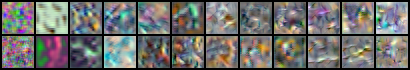
\includegraphics[width=120mm]{images/pseudo_data.png}
  \caption{Pseudo images sampled from generators of different seed, hyperparameters and Teacher-Student pairs at different times during training. As the training develops (from left to right) the images evolve from diverse, random features to shaped patterns. }
  \label{fig:pseudo_images}
\end{figure}

\subsection{Adversarial Belief Matching}

We finally measure the belief matching between teacher and student in both the zero-shot and few-shot settings for both datasets. Figure \ref{fig:transition} depicts the reproduced transition curves for all four cases, and Table \ref{mtetab} shows MTE (equation \ref{MTE}). The performance of the zero-shot model is very similar to the paper, but the transition error of KD-AT is higher. We observe the same pattern as the authors, that similarity in predictions between student and teacher as samples are altered is much worse for KD-AT, despite having comparable test accuracy to the zero-shot model. This is surprising since the procedure is using real data, which KD-AT uses for distillation. We provide a possible explanation for this: The process of manipulating samples towards the student decision boundary might result in images outside the space of real data. Examples of images after $K$ update steps towards the student decision boundary of other classes can be found in Figure \ref{manipulateSamples} of the appendix. The images look like noisy versions of the original class, but are now predicted as another class with almost full certainty by the student. For KD-AT, the student matches the teacher and true labels solely on real samples, whereas the zero-shot student is trained on pseudo-data which is not limited to this space, as is shown in Figure \ref{fig:pseudo_images}. A toy experiment is also conducted in \cite{Micaelli2019ZeroShotKT}, demonstrating how the generator produces samples that follow the decision boundary of the teacher in order to make it more difficult for the student, which could explain the high degree of belief matching in our experiments.

\begin{figure}
  \centering
  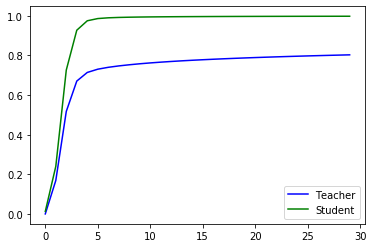
\includegraphics[width=0.31\linewidth]{images/ABM-Teacher-Student-Zero-Shot-CIFAR.png}
  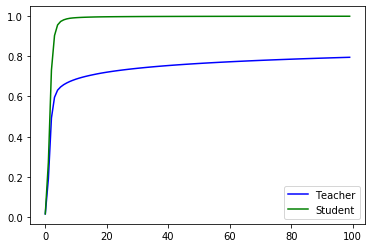
\includegraphics[width=0.31\linewidth]{images/Modified-Zero-Shot_Transition-Curves-CIFAR.png}
  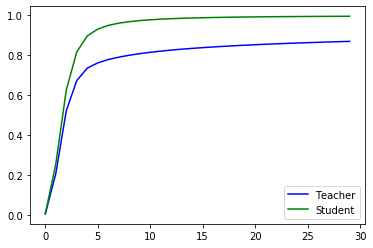
\includegraphics[width=0.31\linewidth]{images/ABM-Teacher-Student-Zero-Shot-SVHN.png}
  %%%%% KD
  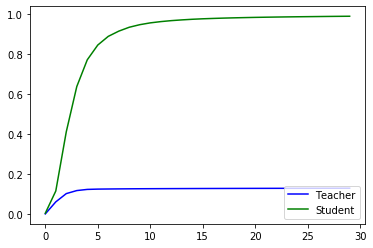
\includegraphics[width=0.31\linewidth]{images/ABM-Teacher-Student-KD-ATT-CIFAR.png}
  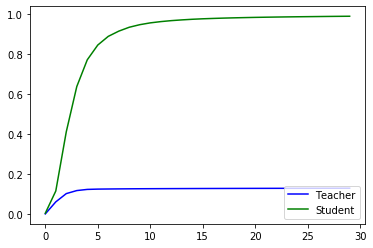
\includegraphics[width=0.31\linewidth]{images/ABM-Teacher-Student-KD-ATT-CIFAR.png}
  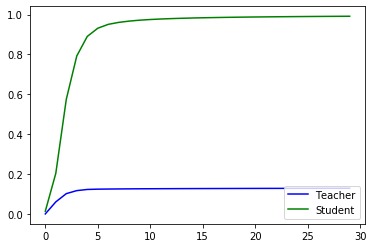
\includegraphics[width=0.31\linewidth]{images/ABM-Teacher-Student-KD-ATT-SVHN.png}
  \caption{Transition curves of teacher and student network when samples from the test sets are manipulated to change their labels. \textbf{Top row}: Zero-Shot on CIFAR(left), Modified Zero-Shot on CIFAR (center) and Zero-Shot on SVHN (right). \textbf{Bottom row}: Corresponding results under the same settings with KD-AT few-shot training. The first two plots are identical of this row are identical.} 
  \label{fig:transition}
\end{figure}

The transition curve plots concerning zero-shot and modified zero-shot on CIFAR show that the deviation between the teacher and student predictions is higher in our method. This is also confirmed by the Mean Transition Error values in Table \ref{mtetab}, and is expected since in our setting more images are used to train the student, and at each batch iteration only one update is performed per image. On the other hand, the original zero-shot method focuses on a single image per batch iteration, where the student in updated $n_s=10$ times on this single image to match the teachers predictions.  

\begin{table}[!h]
    \centering
    \begin{tabular}{cccc}
    \toprule
    \toprule
         \textbf{} & \textbf{Zero-Shot} & \textbf{Modified Zero-Shot}  & \textbf{KD+AT}\\
         \midrule
         SVHN & 0.11 & - & 0.83\\
         CIFAR-10 & 0.18 & 0.22 & 0.81\\
         \bottomrule 
         \bottomrule
    \end{tabular}
    \vspace{0.25cm}
    \caption{Mean Transition errors (MTE) for SVHN and CIFAR-10}
    \label{mtetab}
    \vspace{-0.2cm}

\end{table}

We finally perform an extra ablation study on CIFAR for both the original zero-shot and KD-AT methods, where we replicate the setting of measuring belief matching, with the core difference that samples are updated based on the gradients of the teacher network. This way, the manipulated samples will be the same for both methods. We observe that the performance under this setting is different. The teacher network grows full confidence in the 'new' class after a few updates, while the student network reaches up to a low threshold in its confidence for that class. Thus, mean transition errors are kept high for both cases, with the zero-shot method resulting in a lower error value (0.64) compared to KD-AT (0.78). Plots for the transition curves can be found on section \textbf{D} of the Appendix. 